% Corpus Composition Diagram — Structured Narrative Survey
% Replaces the fabricated PRISMA funnel (1,847→120 numbers had no audit trail).
% This diagram honestly represents the working corpus as described in Section II.
%
% Compile: pdflatex prisma_flowchart_tikz.tex
% Include in main survey with 
\includegraphics{figures/prisma_flowchart_tikz.pdf}

\documentclass[tikz,border=6pt]{standalone}
\usepackage{tikz}
\usetikzlibrary{shapes.geometric,arrows.meta,positioning,shadows}

\definecolor{cblue}{HTML}{003f87}
\definecolor{cred}{HTML}{c0392b}
\definecolor{cgreen}{HTML}{1a7a4a}
\definecolor{corange}{HTML}{e67e22}
\definecolor{lgray}{HTML}{f5f5f5}

\tikzset{
  mainbox/.style={
    rectangle, rounded corners=4pt, draw=cblue, fill=lgray,
    text width=8cm, align=left, font=\small,
    minimum height=1.0cm, drop shadow, inner sep=6pt
  },
  splitbox/.style={
    rectangle, rounded corners=4pt, draw=#1, fill=#1!10,
    text width=5.8cm, align=left, font=\small,
    minimum height=1.0cm, drop shadow, inner sep=6pt
  },
  notebox/.style={
    rectangle, rounded corners=2pt, draw=cred!70, fill=cred!8,
    text width=5.2cm, align=left, font=\scriptsize,
    minimum height=0.8cm, inner sep=4pt
  },
  arrow/.style={-{Latex[length=3mm,width=2mm]}, thick, color=cblue},
  redarrow/.style={-{Latex[length=2.5mm,width=1.5mm]}, color=cred, dashed},
  phaseLabel/.style={font=\footnotesize\bfseries\itshape, color=cblue!70!black}
}

\begin{document}
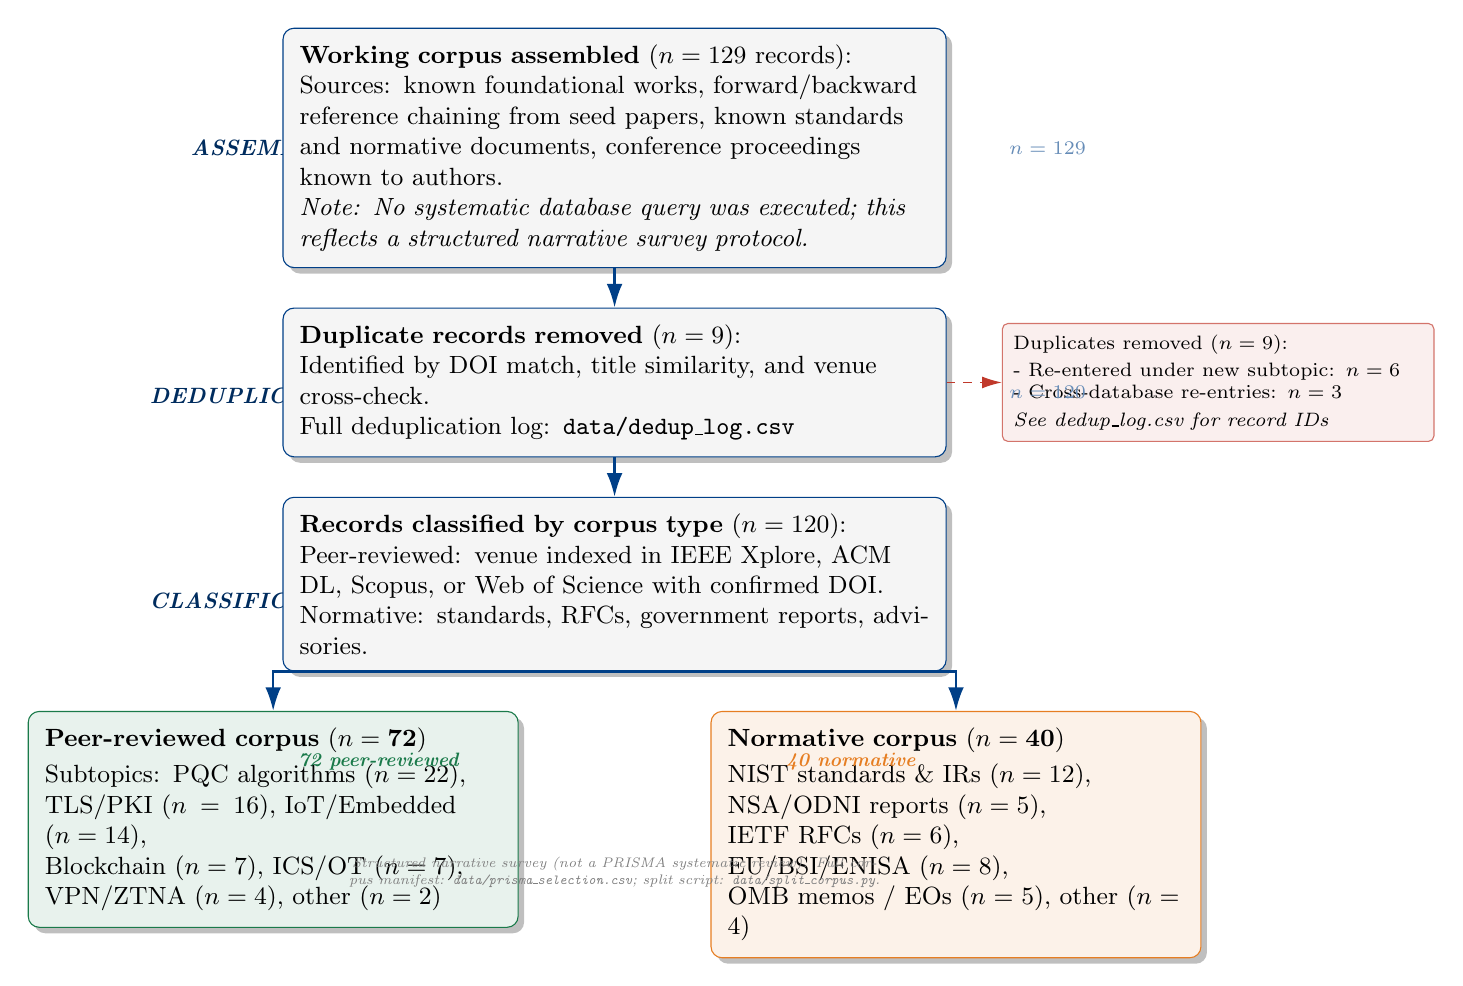
\begin{tikzpicture}[node distance=0.6cm]

%── ASSEMBLY ──────────────────────────────────────────────────────────────────
\node[phaseLabel] at (-4.5, 0) {ASSEMBLY};

\node[mainbox] (asm) at (0,0) {
  \textbf{Working corpus assembled} ($n = 129$ records):\\
  Sources: known foundational works, forward/backward reference
  chaining from seed papers, known standards and normative
  documents, conference proceedings known to authors.\\
  \textit{Note: No systematic database query was executed;
  this reflects a structured narrative survey protocol.}
};

%── DEDUPLICATION ─────────────────────────────────────────────────────────────
\node[phaseLabel, below=1.4cm of asm, xshift=-4.5cm] {DEDUPLICATION};

\node[mainbox, below=0.5cm of asm] (dedup) {
  \textbf{Duplicate records removed} ($n = 9$):\\
  Identified by DOI match, title similarity, and venue cross-check.\\
  Full deduplication log: \texttt{data/dedup\_log.csv}
};

\node[notebox, right=0.7cm of dedup] (ex1) {
  Duplicates removed ($n=9$):\\[2pt]
  - Re-entered under new subtopic: $n=6$\\
  - Cross-database re-entries: $n=3$\\[2pt]
  \textit{See dedup\_log.csv for record IDs}
};
\draw[redarrow] (dedup.east) -- (ex1.west);

%── CORPUS SPLIT ──────────────────────────────────────────────────────────────
\node[phaseLabel, below=1.6cm of dedup, xshift=-4.5cm] {CLASSIFICATION};

\node[mainbox, below=0.5cm of dedup] (split) {
  \textbf{Records classified by corpus type} ($n = 120$):\\
  Peer-reviewed: venue indexed in IEEE Xplore, ACM DL, Scopus,
  or Web of Science with confirmed DOI.\\
  Normative: standards, RFCs, government reports, advisories.
};

%── FINAL CORPORA (side by side) ──────────────────────────────────────────────
\node[phaseLabel, below=1.6cm of split, xshift=-4.5cm] {FINAL CORPORA};

\node[splitbox=cgreen, below left=0.5cm and -3cm of split] (pr) {
  \textbf{Peer-reviewed corpus} ($n = \mathbf{72}$)\\[2pt]
  Subtopics: PQC algorithms ($n=22$),\\
  TLS/PKI ($n=16$), IoT/Embedded ($n=14$),\\
  Blockchain ($n=7$), ICS/OT ($n=7$),\\
  VPN/ZTNA ($n=4$), other ($n=2$)
};

\node[splitbox=corange, below right=0.5cm and -3cm of split] (norm) {
  \textbf{Normative corpus} ($n = \mathbf{40}$)\\[2pt]
  NIST standards \& IRs ($n=12$),\\
  NSA/ODNI reports ($n=5$),\\
  IETF RFCs ($n=6$),\\
  EU/BSI/ENISA ($n=8$),\\
  OMB memos / EOs ($n=5$), other ($n=4$)
};

%── VERTICAL ARROWS ───────────────────────────────────────────────────────────
\draw[arrow] (asm.south) -- (dedup.north);
\draw[arrow] (dedup.south) -- (split.north);
\draw[arrow] (split.south) -| (pr.north);
\draw[arrow] (split.south) -| (norm.north);

%── COUNT ANNOTATIONS ─────────────────────────────────────────────────────────
\node[font=\scriptsize\itshape, color=cblue!60] at (5.5,0)   {$n=129$};
\node[font=\scriptsize\itshape, color=cblue!60] at (5.5,-3.1){$n=120$};
\node[font=\scriptsize\itshape, color=cgreen]   at (-3,-7.8) {\textbf{72 peer-reviewed}};
\node[font=\scriptsize\itshape, color=corange]  at (3,-7.8)  {\textbf{40 normative}};

%── LEGEND NOTE ───────────────────────────────────────────────────────────────
\node[font=\tiny\itshape, color=gray, text width=11cm, align=center]
  at (0,-9.2) {%
  Structured narrative survey (not a PRISMA systematic review).
  Full corpus manifest: \texttt{data/prisma\_selection.csv};
  split script: \texttt{data/split\_corpus.py}.
};

\end{tikzpicture}
\end{document}
